\documentclass[hyperref,UTF8]{ctexart}
\usepackage[dvipdfmx]{graphicx}
\usepackage{gbt7714}
\usepackage{float}
\usepackage{ragged2e}
\usepackage{amsthm}
\usepackage{amssymb}
\usepackage{amsmath}
\usepackage{wrapfig}
\usepackage{tikz}
\usetikzlibrary{arrows.meta}
\usepackage{booktabs}
%\usepackage[a4paper,left=3.18cm,right=3.18cm,top=2.54cm,bottom=2.54cm]{geometry}
\usepackage{tabularx}
\usepackage{array}
\usepackage{caption}
\usepackage{hyperref}
\newcommand{\upcite}[1]{\textsuperscript{\textsuperscript{\cite{#1}}}}
\setCJKfamilyfont{song}{SimSun}
\title{Topological funneling note}
\date{}
\begin{document}
\maketitle
\[
    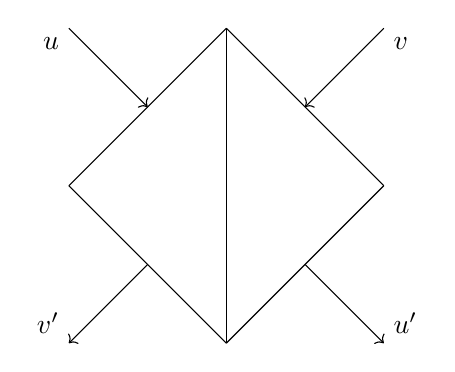
\begin{tikzpicture}
        \coordinate(A) at (-2,0) {};
        \coordinate(B) at (0,2) {};
        \coordinate(C) at (2,0) {};
        \coordinate(D) at (0,-2) {};
        \coordinate(U) at (-2,2) {};
        \coordinate(V) at (2,2) {};
        \node[below left] (O) at (-2,2) {$u$};
        \node[below right] (O) at (2,2) {$v$};
        \draw (A)--(B);
        \draw (C)--(B);
        \draw (C)--(D);
        \draw (A)--(D);
        \draw (B)--(D);
        \draw[->] (U)--(-1,1);
        \draw[->] (V)--(1,1);
        \draw[->] (-1,-1)--(-2,-2);
        \draw[->] (1,-1)--(2,-2);
        \node[above left] (O) at (-2,-2) {$v'$};
        \node[above right] (O) at (2,-2) {$u'$};
    \end{tikzpicture}
\]
对于单个BS分束器,有
\[\begin{pmatrix}
    u'\\v'
\end{pmatrix}=\begin{pmatrix}
    t_u&r_u\\
    r_v&t_v
\end{pmatrix}\begin{pmatrix}
    u\\v
\end{pmatrix}\]
由于能量守恒,上方矩阵是酉的
\begin{figure}[H]
    \centering
    \includegraphics[width = 10cm]{第4页-1.PNG}
\end{figure}
按照上图的摆放,有
\[\begin{pmatrix}
    u_n^m\\v_n^m
\end{pmatrix}=\begin{pmatrix}
    t_u&r_u\\
    r_v&t_v
\end{pmatrix}\begin{pmatrix}
    u_{n-1}^{m-1}\\v_{n+1}^{m-1}
\end{pmatrix}\]
这里的\(m\)随演变增大,可以看作时间,\(n\)是空间的标志,所以这个体系是\(1+1\)维的

按照文献的假定,此时的矩阵为\footnote{此处与文献的记号稍有不同}
\[\begin{pmatrix}
    u_n^m\\v_n^m
\end{pmatrix}=\begin{pmatrix}
    G_u e^{i\varphi_u}&0\\
    0&G_ve^{i\varphi_v}
\end{pmatrix} \begin{pmatrix}
     \cos \beta& i \sin \beta\\
     i \sin \beta& \cos \beta
\end{pmatrix}\begin{pmatrix}
    u_{n-1}^{m-1}\\v_{n+1}^{m-1}
\end{pmatrix}\]
可以写成
\begin{equation}\begin{pmatrix}
    u_n^m\\v_n^m
\end{pmatrix}=\begin{pmatrix}
    G_u e^{i\varphi_u}&0\\
    0&G_ve^{i\varphi_v}
\end{pmatrix} (\mathbf{I} \cos\beta +i\mathbf{\sigma}_x \sin\beta)\begin{pmatrix}
    u_{n-1}^{m-1}\\v_{n+1}^{m-1}
\end{pmatrix} \label{eq:1}
\end{equation}
我们假设光线状态随n(也就是随空间)变化为
\[\begin{pmatrix}
    u_n^m\\v_n^m
\end{pmatrix}=e^{iQ\frac{n}{2}}\begin{pmatrix}
    U^{m}\\V^{m}
\end{pmatrix}\]
这个式子类似平面波假设,此时的矩阵$Q$类似角波数,称为横向Bloch动量(transverse Bloch momentum),代入(\ref{eq:1})中,有
\[\begin{pmatrix}
    U^m\\V^m
\end{pmatrix}=T(Q,G,\varphi,\beta)\begin{pmatrix}
    U^{m-1}\\V^{m-1}
\end{pmatrix}\]
其中
\begin{equation}T(Q,G,\varphi,\beta)=e^{-iQ\frac{n}{2}}\begin{pmatrix}
    G_u e^{i\varphi_u}&0\\
    0&G_ve^{i\varphi_v}
\end{pmatrix} \begin{pmatrix}
    \begin{pmatrix}
        \cos \beta& i \sin \beta
    \end{pmatrix}e^{iQ\frac{n+1}{2}}\\
    \begin{pmatrix}
        i \sin \beta& \cos \beta
    \end{pmatrix}e^{iQ\frac{n-1}{2}}
\end{pmatrix}\label{eq:T}\end{equation}
对于时间演化,我们对称地写出
\[\begin{pmatrix}
    U^{m}\\V^{m}
\end{pmatrix}=e^{i\theta\frac{m}{2}}\begin{pmatrix}
    U\\V
\end{pmatrix}\]
$\theta$称为传播常数(propagation constant)即代表能量 ,有本征方程
\begin{equation}
 e^{i\theta}\begin{pmatrix}
    U\\V
\end{pmatrix}=T(Q,G^2,\varphi^2,\beta^2)T(Q,G^1,\varphi^1,\beta^1)\begin{pmatrix}
    U\\V
\end{pmatrix}\label{eq:eig}
\end{equation}
上标是两个相继的时间步长
\subsection*{均匀晶格}
在均匀晶格中, $G^1=G^2=1,\varphi^1=\varphi^2=0$ ,$\beta^1=\beta^2$是常数\\
由(\ref{eq:T})式,有

\[T(Q,1,0,\beta)=e^{-iQ\frac{n}{2}}\begin{pmatrix}
    \begin{pmatrix}
        \cos \beta& i \sin \beta
    \end{pmatrix}e^{iQ\frac{n+1}{2}}\\
    \begin{pmatrix}
        i \sin \beta& \cos \beta
    \end{pmatrix}e^{iQ\frac{n-1}{2}}
\end{pmatrix}\]
代入本征方程(\ref{eq:eig}),有
\[e^{i\theta}\begin{pmatrix}
    U\\V
\end{pmatrix}=T^2(Q,1,0,\beta)\begin{pmatrix}
    U\\V
\end{pmatrix}=\begin{pmatrix}
    \begin{pmatrix}
        \cos \beta& i \sin \beta
    \end{pmatrix}e^{\frac{1}{2}iQ}\\
    \begin{pmatrix}
        i \sin \beta& \cos \beta
    \end{pmatrix}e^{-\frac{1}{2}iQ}
\end{pmatrix}^2\begin{pmatrix}
    U\\V
\end{pmatrix}\]
\[e^{i\theta}=
\begin{pmatrix}
-\sin ^2\beta+\cos ^2\beta \cos Q+i \cos ^2\beta \sin Q & 
i \sin \beta \cos \beta(1+ \cos Q)-\sin \beta \cos \beta \sin Q \\
i \sin \beta \cos \beta(1+\cos Q)+\sin \beta \cos \beta \sin Q & 
-\sin ^2\beta+\cos ^2\beta \cos Q-i \cos ^2\beta \sin Q 
\end{pmatrix}\]
有
\[\cos \theta = -\sin ^2\beta+\cos ^2\beta \cos Q\]
此即均匀晶格的色散关系
\subsection*{SSH晶格}
在SSH晶体中,$G^1=G^2=1,\varphi^1=\varphi^2=0$,$\beta^1\neq \beta^2$,上方的平方项变为交叉项,有
\[\cos \theta = -\sin\beta^1 \sin\beta^2+\cos\beta^1\cos\beta^2 \cos Q\]
\subsection*{趋肤效应晶格}
在趋肤效应晶格中,$G_u^1=G_u^2=e^{\gamma},G_v^1=G_v^2=e^{-\gamma},\varphi^1=\varphi^2=0$ ,$\beta^1=\beta^2$是常数,有
\[\cos \theta = -\sin ^2\beta+\cos ^2\beta \cos (Q-2i \gamma)\]
\begin{figure}[H]
    \centering
    \includegraphics[width = 10cm]{skin.png}
\end{figure}
\underline{双值SSH模型}

我们来计算zak相,首先有动量空间的酉算子
\[S(Q,\beta^1,\beta^2)=T(Q,1,0,\beta^2)T(Q,1,0,\beta^1)\]
与哈密顿量 $H$ 有下面关系
\[S(Q,\beta^1,\beta^2)=e^{i H(Q,\beta^1,\beta^2)}\]
我们来计算 $S(Q,\beta^1,\beta^2)$ ,根据(\ref{eq:eig})式
\[S=
    \begin{pmatrix}
     -\sin \beta ^1 \sin \beta ^2+e^{i Q} \cos \beta ^1 \cos \beta ^2 & 
     i \sin \beta ^1 \cos\beta ^2+i e^{i Q} \cos \beta ^1 \sin \beta ^2 \\
     i \sin \beta ^1 \cos \beta ^2+i e^{-i Q} \cos \beta ^1 \sin \beta ^2 & 
     -\sin \beta ^1\sin \beta ^2+e^{-i Q} \cos \beta ^1 \cos \beta ^2 \\
    \end{pmatrix}
\]
写成Pauli矩阵的形式
\begin{align*}
    S=&(-\sin \beta ^1 \sin \beta ^2+\cos Q \cos \beta ^1 \cos \beta ^2)\mathbf{I}+i\sigma_x(\sin \beta ^1 \cos\beta ^2+\cos Q \cos \beta ^1 \sin \beta ^2)\\
    &+i\sigma_y(-\sin Q \cos \beta ^1 \sin \beta ^2)+i\sigma_z(\sin Q \cos \beta ^1 \cos \beta ^2)\\
    =&\cos \theta\mathbf{I}+i\vec{n} \cdot \vec{\sigma}\sin \theta
\end{align*}
则有
\[\cos \theta =-\sin \beta ^1 \sin \beta ^2+\cos Q \cos \beta ^1 \cos \beta ^2\]
和
\[\vec{n}=\frac{1}{\sin \theta } \begin{pmatrix}
    \sin \beta ^1 \cos\beta ^2+\cos Q \cos \beta ^1 \sin \beta ^2\\
    -\sin Q \cos \beta ^1 \sin \beta ^2\\
    \sin Q \cos \beta ^1 \cos \beta ^2
\end{pmatrix}\]
注意到
\[\vec{n'}=(e^{-i(\frac{\beta^1}{2}+\frac{\pi}{4})\sigma_y}e^{i\frac{\pi}{4}\sigma_z})\vec{n}=\frac{1}{\sin \theta } \begin{pmatrix}
    -\sin Q \cos \beta ^2 \\
    \cos Q \sin \beta ^1 \cos\beta ^2+\cos \beta ^1 \sin \beta ^2\\
    0
\end{pmatrix}\]
是一个幺正变换,此时的哈密顿量
\[H'=U^\dagger H U\]
此时的本征矢是旋量
\[\psi=\begin{pmatrix}
    \cos \frac{\Theta}{2}\\
    \sin\frac{\Theta}{2} e^{i\phi}
\end{pmatrix}\]
因为$\vec{n'}$在 $xy$平面内,于是 $\Theta=\pi/2$
\[\psi=\frac{\sqrt{2}}{2}\begin{pmatrix}
    1\\
     e^{i\phi}
\end{pmatrix}\]  
令 $e^{i\phi}=f(Q)$ ,则
\[f(Q)=\frac{1}{\sin \theta }(-\sin Q \cos \beta ^2+i(\cos Q \sin \beta ^1 \cos\beta ^2+\cos \beta ^1 \sin \beta ^2))\]
这种情形下,zak相位写成
\[\mathcal{Z} =i\int_{-\pi}^{\pi} \psi^*\frac{\partial}{\partial Q}\psi\mathrm{d}Q=\frac{i}{2}\int_{-\pi}^{\pi}\frac{\partial f(Q)}{\partial Q}f^{-1}(Q)\mathrm{d}Q\]
解得
\begin{align*}
    \mathcal{Z}=&\frac{i}{2\sin ^2\theta}\int_{-\pi}^{\pi}\cos \beta ^2   (\cos Q+i \sin \beta ^1 \sin Q) (i \cos \beta ^1 \sin \beta^2\cos \beta ^2 (\sin Q+i \sin \beta ^1 \cos Q))\mathrm{d}Q\\
    &=- {{\pi  \sin \beta ^1 \cos ^2\beta ^2 }\over{\sin ^2\theta} }
\end{align*}


\end{document}